\chapter{Pruebas}\label{pruebas}

\section{Backend}

El backend de la aplicación es extremadamente pequeño, consta de un único endpoint, un método del servicio y las funciones de cifrar y descifrar en la clase entidad. Por lo tanto, ha sido sencillo obtener una buena cobertura.

\subsection{Listado de pruebas}

\begin{longtable}{|p{0.02\linewidth}|p{0.39\linewidth}|p{0.4\linewidth}|p{0.11\linewidth}|}

    % cabecera
    \hline \textbf{Id} & \textbf{Nombre} & \textbf{Descripción} & \textbf{Ámbito} \\ \hline \endhead
    
    % servicio
    1 & shouldGenerateValidKeyPair & Comprueba que al generar la entidad, ni la entidad ni sus atributos son nulos. & Servicio \\ \hline
    2 & shouldCorrectlyEncodeMessage & Comprueba que el mensaje se haya cifrado correctamente usando la longitud de referencia. & Servicio \\ \hline
    3 & shouldCorrectlyDecodeMessage & Comprueba que el mensaje se haya descifrado correctamente usando el mensaje original de referencia. & Servicio \\ \hline
    
    % controller
    4 & shouldReturnBadRequest & Debe devolver un 400 cuando no se envía el mensaje como parámetro. & Controller \\ \hline
    5 & shouldReturnBadRequestEmptyString & Debe devolver un 400 cuando se envía un mensaje vacío. & Controller \\ \hline
    6 & shouldReturnBadRequestBlankString & Debe devolver un 400 cuando se envía un mensaje en blanco. & Controller \\ \hline
    7 & shouldNotReturnErrorCode & Debe devolver un 200 cuando se hace una petición correcta. & Controller \\ \hline
    8 & shouldReturnErrorCode & Debe devolver un 500 cuando hay un problema interno, es decir, el servicio devuelve una entidad nula. & Controller \\ \hline
    
    \caption{Listado completo de tests del backend}
    \label{tab:tests-backend}
\end{longtable}

\subsection{Cobertura}

La cobertura obtenida ha sido casi total, ahora veremos en concreto qué líneas no están cubiertas por los tests.

\begin{figure}[!ht]
    \centering
    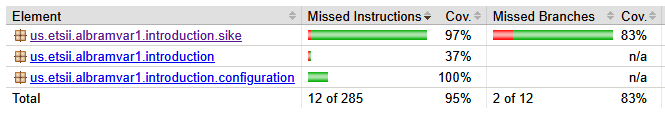
\includegraphics[width=0.85\linewidth]{img/cobertura-modulos.png}
    \caption{Cobertura del proyecto}
    \label{fig:cobertura-modulos}
\end{figure}

Como vemos, la cobertura del módulo 'sike', el que tiene las funcionalidades de generación de claves y cifrado, es de un 97\%, lo que supera el 80\% recomendado.

\begin{figure}[!ht]
    \centering
    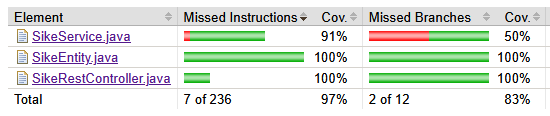
\includegraphics[width=0.75\linewidth]{img/cobertura-clases.png}
    \caption{Cobertura de las clases implementadas}
    \label{fig:cobertura-clases}
\end{figure}

En esta imagen vemos que tanto el controlador como la implementación de la entidad están cubiertas al completo, es sólo el servicio el que no llega al 100\%. Sin embargo, estas líneas no cubiertas son controles explícitos que se han añadido para asegurar el buen funcionamiento interno de la aplicación.

\begin{figure}[!ht]
    \centering
    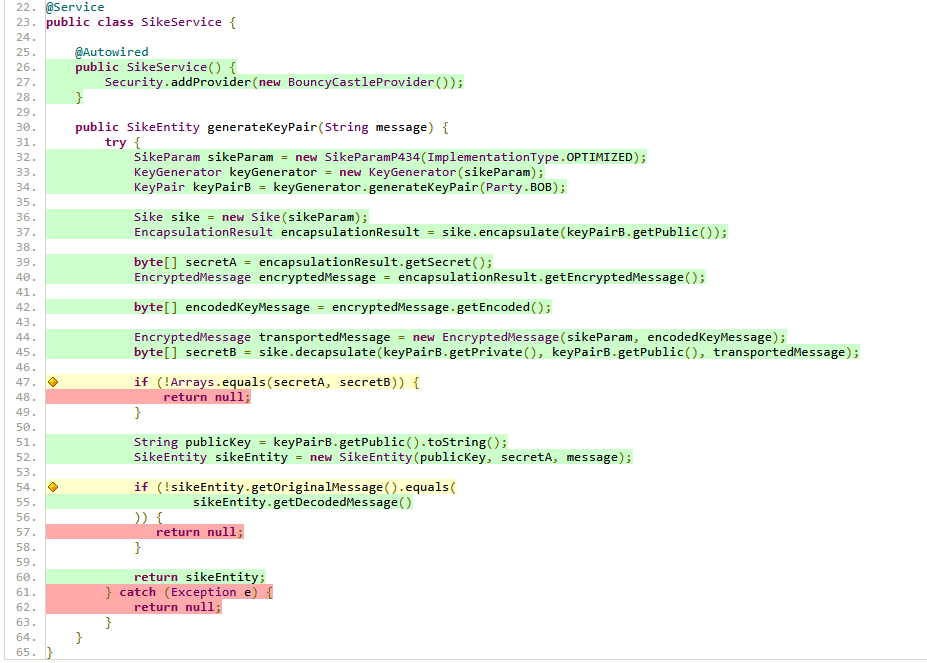
\includegraphics[width=\linewidth]{img/cobertura-servicio.png}
    \caption{Cobertura del servicio}
    \label{fig:cobertura-servicio}
\end{figure}


\section{Frontend}

Aunque el frontend de la aplicación es bastante más grande que el backend, este cumple una función principal de presentación, no teniendo demasiada lógica propia, por lo que obtener una buena cobertura no ha sido difícil.

\subsection{Listado de pruebas}

\begin{longtable}{|p{0.02\linewidth}|p{0.35\linewidth}|p{0.4\linewidth}|p{0.15\linewidth}|}

    % cabecera
    \hline \textbf{Id} & \textbf{Nombre} & \textbf{Descripción} & \textbf{Componente} \\ \hline \endhead
    
    % app
    1 & renders app correctly & Comprueba que que al renderizar la aplicación aparezca la página de inicio. & App \\ \hline

    % about
    2 & renders about section correctly & Comprueba que la sección de información aparezca correctamente. & About \\ \hline
    3 & handle scroll works correctly & Comprueba que la animación de aparición funcione correctamente. & About \\ \hline
    
    % components
    4 & renders message correctly & Comprueba que el mensaje hijo aparezca al renderizar el componente. & AliceToBob \\ \hline
    5 & renders message correctly & Comprueba que el mensaje hijo aparezca al renderizar el componente. & BobToAlice \\ \hline
    6 & renders alice and bob correctly & Comprueba que aparezcan los dos personajes por defecto. & Characters \\ \hline
    7 & hides alice when requested & Comprueba que sólo muestra al personaje deseado, en este caso Bob. & Characters \\ \hline
    8 & hides bob when requested & Comprueba que sólo muestra al personaje deseado, en este caso Alice. & Characters \\ \hline
    9 & renders target text after animation & Comprueba que la animación finaliza con el texto deseado. & DecryptingText \\ \hline
    10 & renders grainient container & Comprueba que el contenedor se renderiza. & Grainient \\ \hline
    11 & renders alice graph view & Comprueba que se renderiza la vista de grafo de Alice por defecto. & GraphView \\ \hline
    12 & renders bob graph view & Comprueba que se renderiza la vista de grafo de Bob cuando se indica. & GraphView \\ \hline
    13 & renders second half correctly & Comprueba que se renderiza la mitad del camino deseado. & GraphView \\ \hline
    14 & load handler is called & Comprueba que el handler ha sido llamado. & GraphView \\ \hline
    15 & renders children with id and classname & Comprueba que los hijos se renderizan correctamente tras la animación. & MotionDiv \\ \hline
    16 & scrolls to top on mount & Comprueba que funciona correctamente al inicio. & ScrollToTop \\ \hline
    17 & renders typewriter container & Comprueba que el contenedor para la animación se renderiza correctamente. & TypewriterText \\ \hline

    % context
    18 & provides initial parameters to children & Comprueba que los valores iniciales se cargan correctamente. & Parameters- Context  \\ \hline

    % footer
    19 & renders footer correctly & Comprueba que el pie de página tiene los componentes necesarios. & Footer \\ \hline

    % hero
    20 & renders hero correctly & Comprueba que la sección hero del inicio contiene a los componentes deseados. & Hero \\ \hline

    % home
    21 & renders home correctly & Comprueba que la página de inicio contiene sus tres componentes principales. & Home \\ \hline

    % navbar
    22 & renders links correctly & Comprueba que la barra de navegación incluye los links necesarios. & Navbar \\ \hline
    23 & home link click & Comprueba la funcionalidad del enlace y la aplicación de estilos. & Navbar \\ \hline
    24 & proof of identity link click & Comprueba la funcionalidad del enlace y la aplicación de estilos. & Navbar \\ \hline
    25 & key exchange link click & Comprueba la funcionalidad del enlace y la aplicación de estilos. & Navbar \\ \hline
    26 & encryption link click & Comprueba la funcionalidad del enlace y la aplicación de estilos. & Navbar \\ \hline
    27 & about link click & Comprueba la funcionalidad del enlace y la aplicación de estilos. & Navbar \\ \hline
    28 & i18n renders in navbar & Comprueba que las opciones de idioma están disponibles en la barra de navegación. & Navbar \\ \hline

    % protocols
    29 & renders protocols correctly & Comprueba que el menú de protocolos aparece correctamente. & Protocols \\ \hline
    30 & handle scroll works correctly & Comprueba que la animación de aparición funciona correctamente. & Protocols \\ \hline

    % protocol view
    31 & renders protocol view correctly & Comprueba que la vista de protocolo contiene los elementos necesarios. & ProtocolView \\ \hline
    32 & renders player correctly & Comprueba que los controles de reproductor aparecen correctamente. & ProtocolView \\ \hline
    33 & player button toggles play & Comprueba que el botón de play inicia la presentación. & ProtocolView \\ \hline
    34 & player button increments and decrements steps & Comprueba el funcionamiento de los controles del reproductor. & ProtocolView \\ \hline
    35 & start button toggles play & Comprueba que el botón de inicio comienza la presentación. & ProtocolView \\ \hline
    36 & renders start controls for proof-of-identity & Comprueba que la vista se renderiza correctamente para el protocolo de prueba de identidad. & ProtocolView \\ \hline
    37 & renders start controls for key-exchange & Comprueba que la vista se renderiza correctamente para el protocolo de intercambio de clave. & ProtocolView \\ \hline
    38 & renders start controls for encryption & Comprueba que la vista se renderiza correctamente para el protocolo de cifrado. & ProtocolView \\ \hline

    % proof of identity
    39 & renders step 1 correctly & Comprueba que el paso se renderiza correctamente. & ProofOfIdentity \\ \hline
    40 & renders step 2 correctly & Comprueba que el paso se renderiza correctamente. & ProofOfIdentity \\ \hline
    41 & renders step 3 correctly & Comprueba que el paso se renderiza correctamente. & ProofOfIdentity \\ \hline
    42 & renders step 4 correctly & Comprueba que el paso se renderiza correctamente. & ProofOfIdentity \\ \hline
    43 & renders step 5 correctly & Comprueba que el paso se renderiza correctamente. & ProofOfIdentity \\ \hline
    44 & step 5 random bit & Comprueba que la animación de bit aleatorio funciona correctamente. & ProofOfIdentity \\ \hline
    45 & renders step 6 correctly & Comprueba que el paso se renderiza correctamente. & ProofOfIdentity \\ \hline

    % key exchange
    46 & renders step 1 correctly & Comprueba que el paso se renderiza correctamente. & KeyExchange \\ \hline
    47 & renders step 2 correctly & Comprueba que el paso se renderiza correctamente. & KeyExchange \\ \hline
    48 & renders step 3 correctly & Comprueba que el paso se renderiza correctamente. & KeyExchange \\ \hline
    49 & renders step 4 correctly & Comprueba que el paso se renderiza correctamente. & KeyExchange \\ \hline
    50 & renders step 5 correctly & Comprueba que el paso se renderiza correctamente. & KeyExchange \\ \hline
    51 & renders step 6 correctly & Comprueba que el paso se renderiza correctamente. & KeyExchange \\ \hline
    52 & renders step 7 correctly & Comprueba que el paso se renderiza correctamente. & KeyExchange \\ \hline

    % encryption
    53 & renders step 1 correctly & Comprueba que el paso se renderiza correctamente. & Encryption \\ \hline
    54 & step 1 handle change & Comprueba que el mensaje se guarda correctamente cuando se escribe en el campo de entrada. & Encryption \\ \hline
    55 & step 1 handle change error & Comprueba que la comprobación de texto funciona correctamente. & Encryption \\ \hline
    56 & renders step 2 correctly & Comprueba que el paso se renderiza correctamente. & Encryption \\ \hline
    57 & step 2 on click & Comprueba que al hacer click se llama al backend. & Encryption \\ \hline
    58 & renders step 3 correctly & Comprueba que el paso se renderiza correctamente. & Encryption \\ \hline
    59 & renders step 4 correctly & Comprueba que el paso se renderiza correctamente. & Encryption \\ \hline
    60 & renders step 5 correctly & Comprueba que el paso se renderiza correctamente. & Encryption \\ \hline
    61 & renders step 6 correctly & Comprueba que el paso se renderiza correctamente. & Encryption \\ \hline
    
    \caption{Listado completo de tests del frontend}
    \label{tab:tests-frontend}
\end{longtable}


\subsection{Cobertura}

La cobertura obtenida con estos tests ha sido bastante buena, aunque no perfecta. En total ha sido de casi un 90\%, y la mitad exacta (seis de los 12 componentes cuya cobertura se comprueba) tienen una cobertura del 100\%.

Hay dos componentes en concreto que tienen una cobertura nula y estos son el index.js y el i18n.js. Esta falta de cobertura se debe a desconocimiento de cómo diseñar una suite de tests orientada a ellos además de un testing informal que se ha realizado a lo largo del desarrollo y también justo antes de hacer cualquier subida.

En la siguiente página se incluye el desglose completo de la cobertura obtenida.

\begin{figure}[!ht]
    \centering
    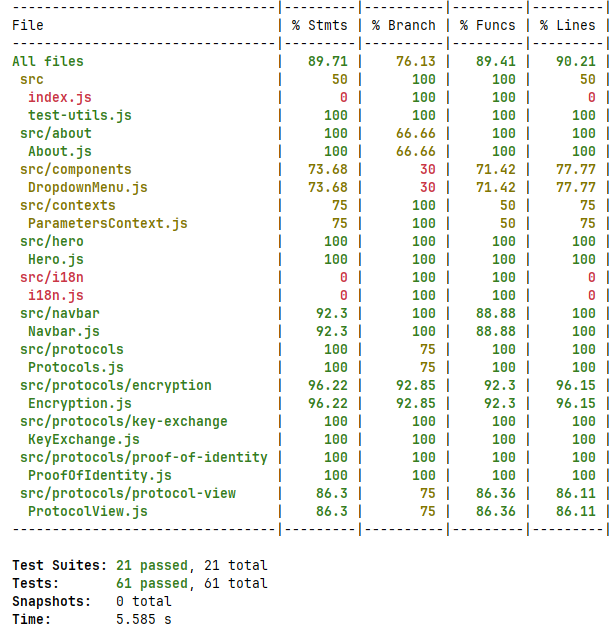
\includegraphics[width=\linewidth]{img/cobertura-frontend.png}
    \caption{Cobertura obtenida}
    \label{fig:cobertura-frontend}
\end{figure}